Desde que nació en 2013, Docker ha ido creciendo y con ello las aplicaciones
directas que ha encontrado en el mercado.

\subsubsection*{\textit{Sandboxing}}
Una de las principales ventajas que otorgó Docker desde su nacimiento fue el de
aislar las aplicaciones entre sí y, por consiguiente, ofrecer un entorno de
``caja de arena'' (\textit{sandbox}) en donde ejecutar nuestras aplicaciones
(o aplicaciones inseguras) con cierta confianza \cite{yegulalpWhatDockerSpark2019}.

Es cierto que esta característica ya estaba asentada con las máquinas virtuales,
y funcionaba correctamente y de forma efectiva. Sin embargo, el tiempo de despliegue
y lentitud de una máquina virtual hacía que usarlas para este propósito fuese
costoso y no resultase interesante.

Con los contenedores se puede tener un entorno aislado que funciona igual de rápido
que una aplicación nativa con unos tiempos de despliegue y uso de recursos limitado.
Como se ha visto anteriormente, el motor de ejecución de Docker tiene el control sobre
un montón de componentes virtuales y reales que permiten, entre otros, limitar y
restringir el acceso a los recursos \textit{hardware} del dispositivo. Bajo esta
premisa, un contenedor puede usar solo cierta cantidad de CPU, RAM o red y que
cambie en tiempo de ejecución.

\subsubsection*{Portabilidad}
Otra de las características fundamentales de los contenedores es la
capacidad de encapsular un \textit{software} y todas
sus dependencias. Esto convierte a los contenedores en una gran solución portable:
sabemos que si una aplicación funciona en Docker en un equipo Linux, funcionará en
Docker de otro equipo Linux exactamente igual, sin necesidad de realizar ningún
cambio e indiferentemente de la distribución.

Con la llegada de WSL2, el kernel de Linux se introdujo al completo dentro de las
máquinas Windows 10, permitiendo que Docker se pudiera ejecutar de ``forma nativa''\cite{DockerDesktopWSL2021}. Con esto, la limitación anterior
se elimina y los contenedores diseñados para Linux funcionarán también en Windows.

Esto ha tenido una repercusión directa con el auge de los sistemas basados en la
nube, los cuales a veces resultaban complejos y tediosos. Con los contenedores, una
aplicación que un desarrollador ejecuta \textit{on-premise} en su equipo puede
ser fácilmente desplegada a un entorno \textit{cloud} sin necesidad de preocuparse
si cumple los requisitos o instala las dependencias. La única restricción es que el
entorno \textit{cloud} al que se mueva soporte Docker.

\subsubsection*{Arquitectura de composición}
Una gran mayoría de aplicaciones que se ejecutan actualmente están ejecutándose sobre
una pila de aplicaciones: servidor web, base de datos, caché en memoria, gestión de
\textit{logs}, etc. La pregunta es, ¿qué sucedería si se encapsula cada una de esas
aplicaciones en un contenedor?

Así nace la arquitectura de microservicios, tan popular y estandarizada hoy en día.
Un microservicio define un elemento único de una aplicación (que puede ser usado
entre $1 \dots n$ veces) el cual acelera y facilita las labores de desarrollo de una
aplicación. Entre otras ventajas, un microservicio puede ser actualizado, reemplazado,
eliminado o modificado sin afectar al resto de microservicios que componen una
aplicación. Esta alternativa se ha asentado como la solución ideal a las aplicaciones
monolíticas monstruosas, que lo engloban todo (como XAMPP) ya que han demostrado ser
mucho más fáciles de mantener y desarrollar.

\subsubsection*{Escalado y orquestación}
Aprovechando la arquitectura de microservicios y contenedores, existen
técnicas de escalado y orquestación automáticas basadas en Docker y contenedores.

De esta manera, en picos de conexión se despliegan automáticamente más contenedores
que gestionan entre ellos las peticiones entrantes y salientes. Cuando las solicitudes
bajan, los contenedores en deshuso desaparecen para dejar de usar recursos.

Entre las herramientas más sonadas para la gestión de contenedores está
Kubernetes, desarrollado por Google. La idea de orquestación nace a raíz de esta
empresa que empieza a invertir cantidades millonarias de dinero en contenedores porque
le ve un nuevo potencial: las comunicaciones vía Internet de los contenedores.
Hasta ahora solo hemos visto un modelo de arquitectura: un cliente Docker que ejecuta
uno o varios contenedores. Sin embargo, con la aparición de los microservicios y la
orquestación, y dadas las características de red de los contenedores, se abre la
posibilidad de que múltiples clientes Docker en máquinas físicamente distintas puedan
estar ejecutándose de forma simultánea y compartiendo datos entre ellos fácilmente.

Debido a las capas de aislamiento de Docker, esta comunicación no es sencilla: no sirve
con comunicar dos direcciones IP. Sin embargo, utilizando un motor de Docker distribuído
se pueden realizar las conexiones como si de una LAN se tratase, cuando en realidad se
está usando una red \textit{overlay}. Esto se muestra en la figura \ref{fig:docker-network}:

\begin{figure}[H]
    \centering
    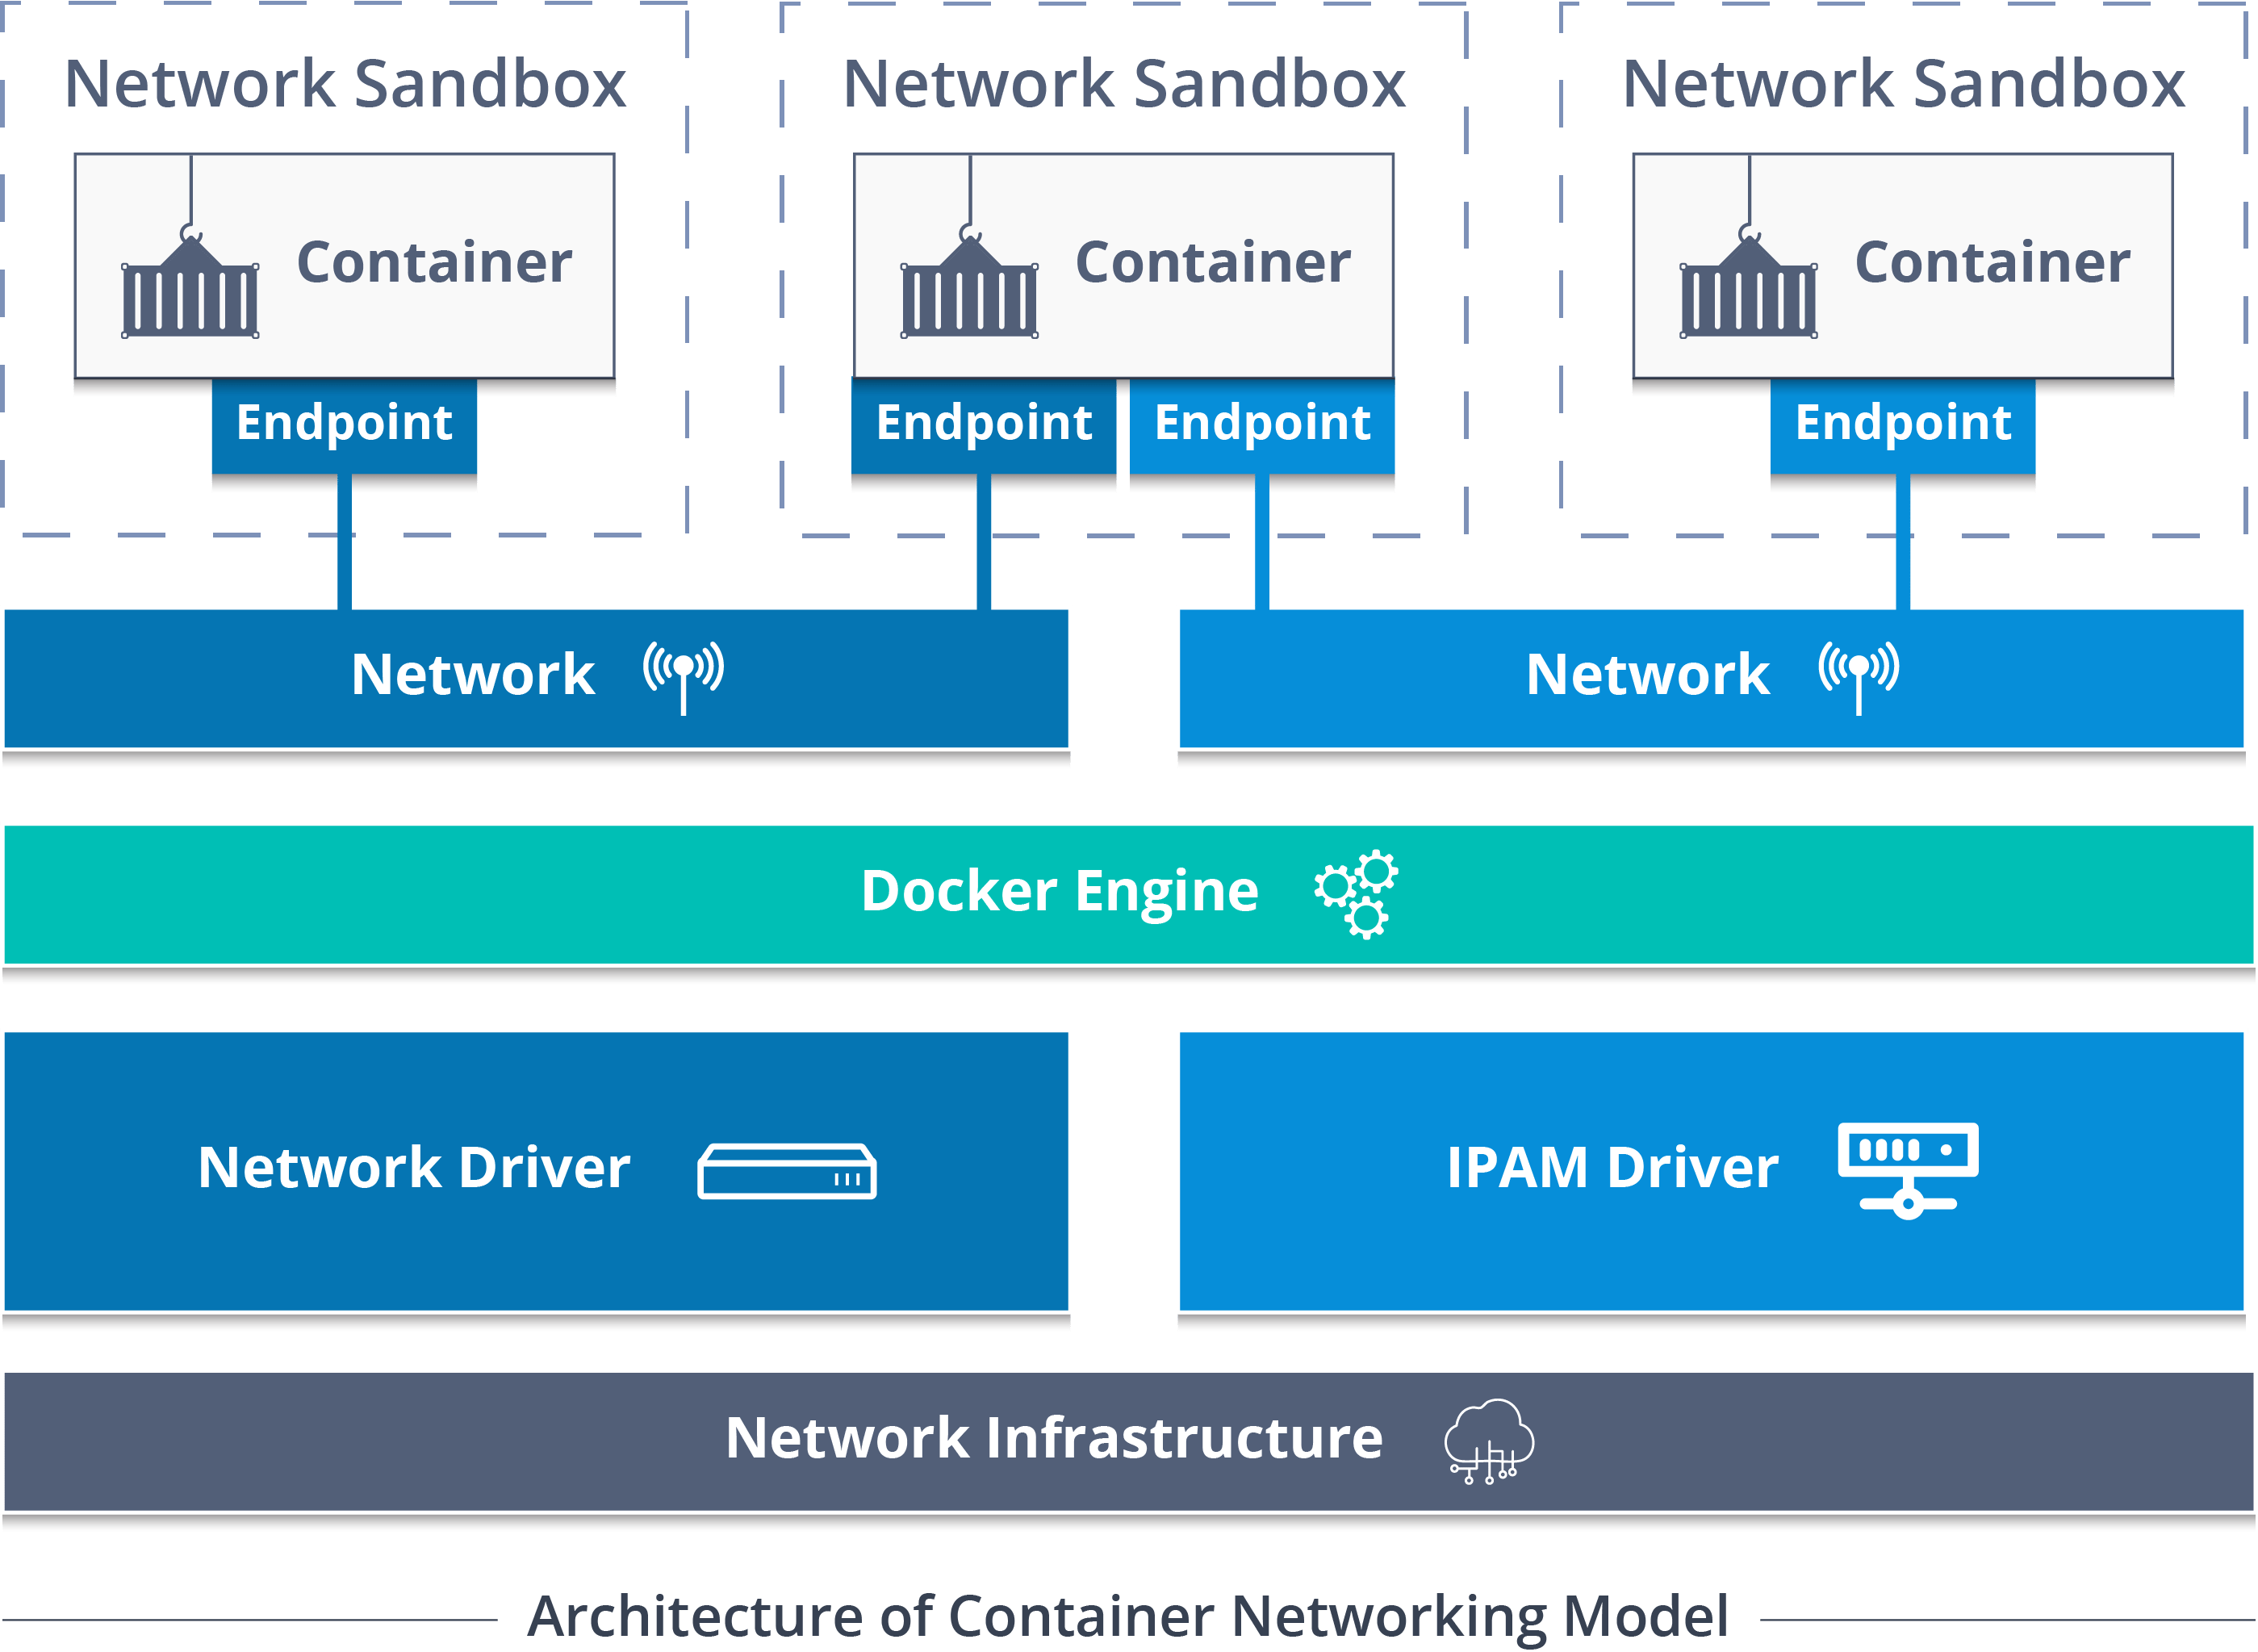
\includegraphics[width=.7\linewidth]{pictures/docker-networking.png}
    \caption{Comunicación entre contenedores usando el motor de Docker \cite{kulshresthaDockerNetworkingExplore2020}.}
    \label{fig:docker-network}
\end{figure}

Con todas estas ideas en mente, es evidente que Docker ofrece soluciones fáciles
y sencillas para escalar automáticamente aplicaciones alrededor de un clúster de
nodos distribuído por el mundo.

\noindent\rule{\linewidth}{.2pt}

Muchas de las aplicaciones de Docker surgen en el mundo DevOps, en donde la mayoría de
herramientas de integración continua (CI) y despliegue continuo (CD) han migrado sus
infraestructuras hacia Docker. Con esto se consigue que los tests y las compilaciones
se hagan de forma sencilla con contenedores de un solo uso.

Otra aplicación directa son las arquitecturas \textit{cloud}, en donde antes había que
configurar cientos de parámetros para desplegar una aplicación web basada en PHP y 
MySQL y ahora basta con usar uno o varios contenedores que agrupen las funcionalidades
que necesitamos.

Por otra parte, gracias a los contenedores los tiempos de desarrollo se han agilizado
mucho. Antes, por ejemplo, una aplicación requería de compilar ciertos paquetes
y realizar ciertas instalaciones que llevaban mucho tiempo. Con Docker, se exponen
las librerías necesarias y se trabaja directamente con aquello que se necesita,
sin necesidad de dedicar tiempo a esas tareas.
